\documentclass[11pt, aspectratio=169, xcolor=table]{beamer}
\usepackage[utf8]{inputenc}
\usepackage[T1]{fontenc}
\usepackage{graphicx}
\usepackage{hyperref}
\usepackage{lmodern}
\usepackage[spanish]{babel}
\usepackage{pdfrender}
\usepackage{xcolor}
\usepackage{ragged2e}
\usepackage[version=4]{mhchem}
\usepackage{siunitx}
\renewcommand{\raggedright}{\justifying}
\usepackage{smartdiagram}
\usetheme{Berlin}

\author{Prof. Daniel Muñoz \\
	\texttt{daniel.munoz3@mail.udp}.cl
}
\title{Química Unidad 4}
\subtitle{Química del agua. Desde la industria hasta el medioambiente}

\begin{document}

\maketitle

\section{Unidades de concentración física (porcentajes p/p, p/v y v/v). Cálculos en disoluciones con concentraciones molares.}

\begin{frame}[allowdisplaybreaks]
	\frametitle{Introducción}
	\begin{columns}
		\begin{column}{.5\textwidth}
			\begin{itemize}[<+->]
				\item ¿Qué es una disolución? $\rightarrow$ Mezcla homogénea de soluto y disolvente.
				\item Componentes: soluto (en menor cantidad) y disolvente (en mayor cantidad).
				\item Ejemplos cotidianos: suero fisiológico, jugos, soluciones limpiadoras.
				\item Importancia de medir ``cuánto'' soluto hay en una disolución.
				\item Las distintas formas de expresar concentración responden a diferentes contextos: industria, laboratorio, medioambiente.
			\end{itemize}
		\end{column}

		\begin{column}{.5\textwidth}
			\begin{figure}[ht]
				\centering
				\includegraphics[width=\textwidth]{../img/mezcla.png}
				\caption{\label{fig:label} Mezcla a nivel microscópico}
			\end{figure}

		\end{column}
	\end{columns}
\end{frame}

\begin{frame}[allowdisplaybreaks]
	\frametitle{Unidades de Concentración Físicas}
	\begin{columns}
		\begin{column}{.5\textwidth}
			\textbf{Definiciones:}
			\begin{itemize}[<+->]
				\small
				\item \% m/m (p/p): (masa soluto / masa disolución) $\times$  100
				\item Ej.: 10 g NaCl en 90 g \ce{H2O} $\rightarrow$ disolución 10 \% p/p
				\item \% m/v (p/v): (masa soluto / volumen disolución) $\times$ 100
				\item Ej.: 5 g glucosa en 100 mL solución $\rightarrow$ 5 \% p/v
				\item \% v/v: (volumen soluto / volumen disolución) $\times$ 100
				\item Ej.: 40 mL etanol en 100 mL disolución $\rightarrow$ 40 \% v/v
			\end{itemize}
		\end{column}

		\begin{column}{.5\textwidth}
			\begin{block}{Usos}
				\begin{itemize}[<+->]
					\item p/p: común en industria alimentaria y farmacéutica.
					\item p/v: común en soluciones de laboratorio.
					\item v/v: común en soluciones líquidas miscibles (alcohol, perfumes).
				\end{itemize}
			\end{block}
		\end{column}
	\end{columns}
\end{frame}

\begin{frame}[allowdisplaybreaks]
	\frametitle{Ejemplo}
	\begin{columns}
		\begin{column}{.5\textwidth}
			\begin{exampleblock}{Problema}
				¿Cuál es el \% p/v de una disolución con 5,0 g de NaCl en 250 mL?
			\end{exampleblock}
		\end{column}

		\begin{column}{.5\textwidth}

		\end{column}
	\end{columns}
\end{frame}

\begin{frame}[allowdisplaybreaks]
	\frametitle{Concentración Molar}
	\begin{columns}
		\begin{column}{.5\textwidth}
			\textbf{Definición:}
			\begin{itemize}[<+->]
				\item Molaridad (M) = moles de soluto / litros de disolución.
				\item Pasos clave:
				      \begin{itemize}[<+->]
					      \item Calcular moles: n = masa / peso molecular (PM)
					      \item Convertir volumen a litros
					      \item Aplicar fórmula
				      \end{itemize}
			\end{itemize}
		\end{column}

		\begin{column}{.5\textwidth}
			\begin{block}{Importancia}
				\begin{itemize}[<+->]
					\item Base para cálculos estequiométricos y preparación precisa de soluciones.
					\item Permite relacionar directamente masa $\leftrightarrow$ volumen $\leftrightarrow$ cantidad de sustancia.
					\item Unidades: \unit{mol/L} o \unit{\mol\per\litre}
				\end{itemize}
			\end{block}
		\end{column}
	\end{columns}
\end{frame}

\begin{frame}[allowdisplaybreaks]
	\frametitle{Ejemplo 2}
	\begin{columns}
		\begin{column}{.5\textwidth}
			\begin{exampleblock}{Problema}
				Se tienen 100 mL de disolución con 0,56 g de KOH. Determine la concentración molar de la disolución
			\end{exampleblock}

		\end{column}

		\begin{column}{.5\textwidth}

		\end{column}
	\end{columns}
\end{frame}

\begin{frame}[allowdisplaybreaks]
	\frametitle{Ejemplo 3}
	\begin{columns}
		\begin{column}{.5\textwidth}
			\begin{exampleblock}{Problema}
				Determine la concentración molar de una solución de 100 mL de disolución con 0,740 g de \ce{Ca(OH)2}
			\end{exampleblock}

		\end{column}

		\begin{column}{.5\textwidth}

		\end{column}
	\end{columns}

\end{frame}

\section{Definición, Expresión e interpretación de la constante de equilibrio en reacciones ácido base}

\begin{frame}[allowdisplaybreaks]
	\frametitle{Introducción al equilibrio}
	\begin{columns}
		\begin{column}{.5\textwidth}
			\begin{itemize}[<+->]
				\item Un equilibrio químico ocurre cuando la velocidad de la reacción directa es igual a la inversa.
				\item Las concentraciones de reactantes y productos se mantienen constantes en el tiempo.
				\item No implica que reactantes y productos estén en igual cantidad.
				\item Ejemplo cotidiano: Corrosión: Lo que se oxida puede recuperarse: \ce{4Fe + 3O2 -> 2Fe2O3}
			\end{itemize}
		\end{column}

		\begin{column}{.5\textwidth}
			\begin{figure}[ht]
				\centering
				\includegraphics[width=0.6\textwidth]{../img/equilibrio1.jpeg}
				\caption{Existen productos que nos permiten eliminar el óxido.}
			\end{figure}

		\end{column}
	\end{columns}
\end{frame}

\begin{frame}[allowdisplaybreaks]
	\frametitle{Constante de equilibrio}
	\begin{columns}
		\begin{column}{.5\textwidth}
			\begin{itemize}[<+->]
				\small
				\item En una reacción en equilibrio la \textit{velocidad} a la que ocurre:
				      \begin{itemize}[<+->]
					      \small
					      \item la reacción directa:  \ce{2H+(ac) + CO3^2-(ac) -> H2CO3(ac)} es igual a
					      \item la reacción inversa: \ce{H2CO3(ac) -> 2H+(ac) + CO3^2-(ac)} y por tanto
					      \item lo escribimos \ce{2H+(ac) + CO3^2-(ac) <=> H2CO3(ac)}
				      \end{itemize}
				\item El \textit{estado de equilibrio} se cuantifica de la siguiente forma para la reacción ejemplo:
				\item $\frac{[\ce{H2CO3}]}{[\ce{H+}]^{2}[\ce{CO3^2-}]^{2}}$
			\end{itemize}
		\end{column}

		\begin{column}{.5\textwidth}
			\begin{figure}[ht]
				\centering
				\includegraphics[width=.6\textwidth]{../img/vel-eq.png}
				\caption{\label{fig:label} Después de un tiempo de iniciada la reacción las velocidades directa e inversa se igualan}
			\end{figure}

		\end{column}
	\end{columns}
\end{frame}

\begin{frame}[allowdisplaybreaks]
	\frametitle{Constante de equilibrio II}
	\begin{columns}
		\begin{column}{.5\textwidth}
			\begin{itemize}[<+->]
				\item Solo se incluyen las especies en estado acuoso o gaseoso (nunca líquidos puros como el agua).
				\item El valor de K indica hacia qué lado se favorece el equilibrio:
				      \begin{itemize}
					      \item K >> 1 $\rightarrow$ \textit{equilibrio está desplazado} a los productos
					      \item K << 1 $\rightarrow$ \textit{equilibrio está desplazado} a los reactantes
				      \end{itemize}
			\end{itemize}
		\end{column}
		\begin{column}{.5\textwidth}
			\begin{figure}[ht]
				\centering
				\includegraphics[width=\textwidth]{../img/interpretacion-cte.png}
				\caption{\label{fig:label} Interpretación de la constante}
			\end{figure}
		\end{column}
	\end{columns}
\end{frame}

\begin{frame}[allowdisplaybreaks]
	\frametitle{Jacobus Van ’t Hoff}
	\begin{columns}
		\begin{column}{.5\textwidth}
			\begin{itemize}[<+->]
				\item Químico neerlandés 1852 - 1911.
				\item Estudió Química en la Universidad Bonn, Paris, dónde coincidió con \textit{Kekulé} como su profesor.
				\item Van ’t Hoff desarrolló la teoría del equilibrio químico y su relación con la energía. Entre muchas otras más.
				\item Estableció cómo las concentraciones se relacionan con el equilibrio mediante ecuaciones cuantitativas.
				\item Premio Nobel de Química 1901.
			\end{itemize}
		\end{column}

		\begin{column}{.5\textwidth}
			\begin{figure}[ht]
				\centering
				\includegraphics[height=0.6\textheight]{../img/vanthoff.png}
				\caption{\label{fig:label} Foto aprox. 1900}
			\end{figure}

		\end{column}
	\end{columns}
\end{frame}

\begin{frame}[allowdisplaybreaks]
	\frametitle{Ejemplo}
	\begin{columns}
		\begin{column}{.5\textwidth}
			\begin{exampleblock}{Acidificación de los océanos}
				Exprese la constante de equilibrio de la reacción:
				\ce{CO2(g) + H2O(l) <=> H2CO3}
			\end{exampleblock}

		\end{column}

		\begin{column}{.5\textwidth}

		\end{column}
	\end{columns}
\end{frame}

\section{Predicción del desplazamiento de un equilibrio ácido base en función de las concentraciones de los reactantes o productos}

\begin{frame}[allowdisplaybreaks]
	\frametitle{Predicción del desplazamiento del equilibrio}
	\begin{columns}
		\begin{column}{.5\textwidth}
			\begin{itemize}[<+->]
				\item El equilibrio se puede alterar cambiando:
				      \begin{itemize}[<+->]
					      \item [Reactantes]: desplazamiento hacia productos.
					      \item [Productos]: desplazamiento hacia reactantes.
					      \item Temperatura o presión.
				      \end{itemize}
				\item Principio de Le Châtelier: el sistema tiende a oponerse al cambio impuesto.
			\end{itemize}
		\end{column}

		\begin{column}{.5\textwidth}
			\begin{itemize}[<+->]
				\item $\uparrow P$ como respuesta la rx. : \ce{R <<=> P}
				\item $\uparrow R$ como respuesta la rx. : \ce{R <=>> P}
			\end{itemize}
		\end{column}
	\end{columns}
\end{frame}

\begin{frame}[allowdisplaybreaks]
	\frametitle{Ejemplo. Desplazamiento por aumento de concentración}
	\begin{exampleblock}{Determine hacia dónde se desplaza el equilibrio}
		Sea la reacción: \ce{NH3(ac) + H2O(l) <=> NH4+(ac) + OH-(ac)} responda para:
		\begin{enumerate}
			\item Agregamos \ce{NH3}
			\item Agregamos \ce{NH4+}
		\end{enumerate}
	\end{exampleblock}
\end{frame}

\begin{frame}[allowdisplaybreaks]
	\frametitle{Ejemplo. Reacción en equilibrio gaseoso}
	\begin{exampleblock}{Responda}
		Sea la reacción \ce{NO2(g) + O2(g) <=> NO(g) + O3(g)}
		\begin{enumerate}
			\item ¿Tipo de equilibrio?
			\item Exprese la K
			\item Si se aumenta [\ce{O2}].
		\end{enumerate}

	\end{exampleblock}
\end{frame}

\section{Definición de pH y cálculo de pH de ácidos y bases fuertes}

\begin{frame}[allowdisplaybreaks]
	\frametitle{¿Qué es un ácido y una base?}
	\begin{columns}
		\begin{column}{.5\textwidth}
			\begin{itemize}[<+->]
				\small
				\item Es conocido en la cultura popular el concepto de ácido, pero ¿Qué es un ácido?
				\item En química existen muchas definiciones de ácidos y bases, la primera y más sencilla de ellas dice:.
				\item \textit{Un ácido sustancia que libera iones \ce{H+} en agua.}
				\item Ejemplo: \ce{HCl(ac) -> H+(ac) + Cl-(ac)}
				\item \textit{Una base sustancia que libera iones \ce{OH-} en agua.}
				\item Ejemplo: \ce{NaOH(s) -> Na+(ac) + OH-(ac)}
			\end{itemize}
		\end{column}

		\begin{column}{.5\textwidth}
			\begin{figure}[ht]
				\centering
				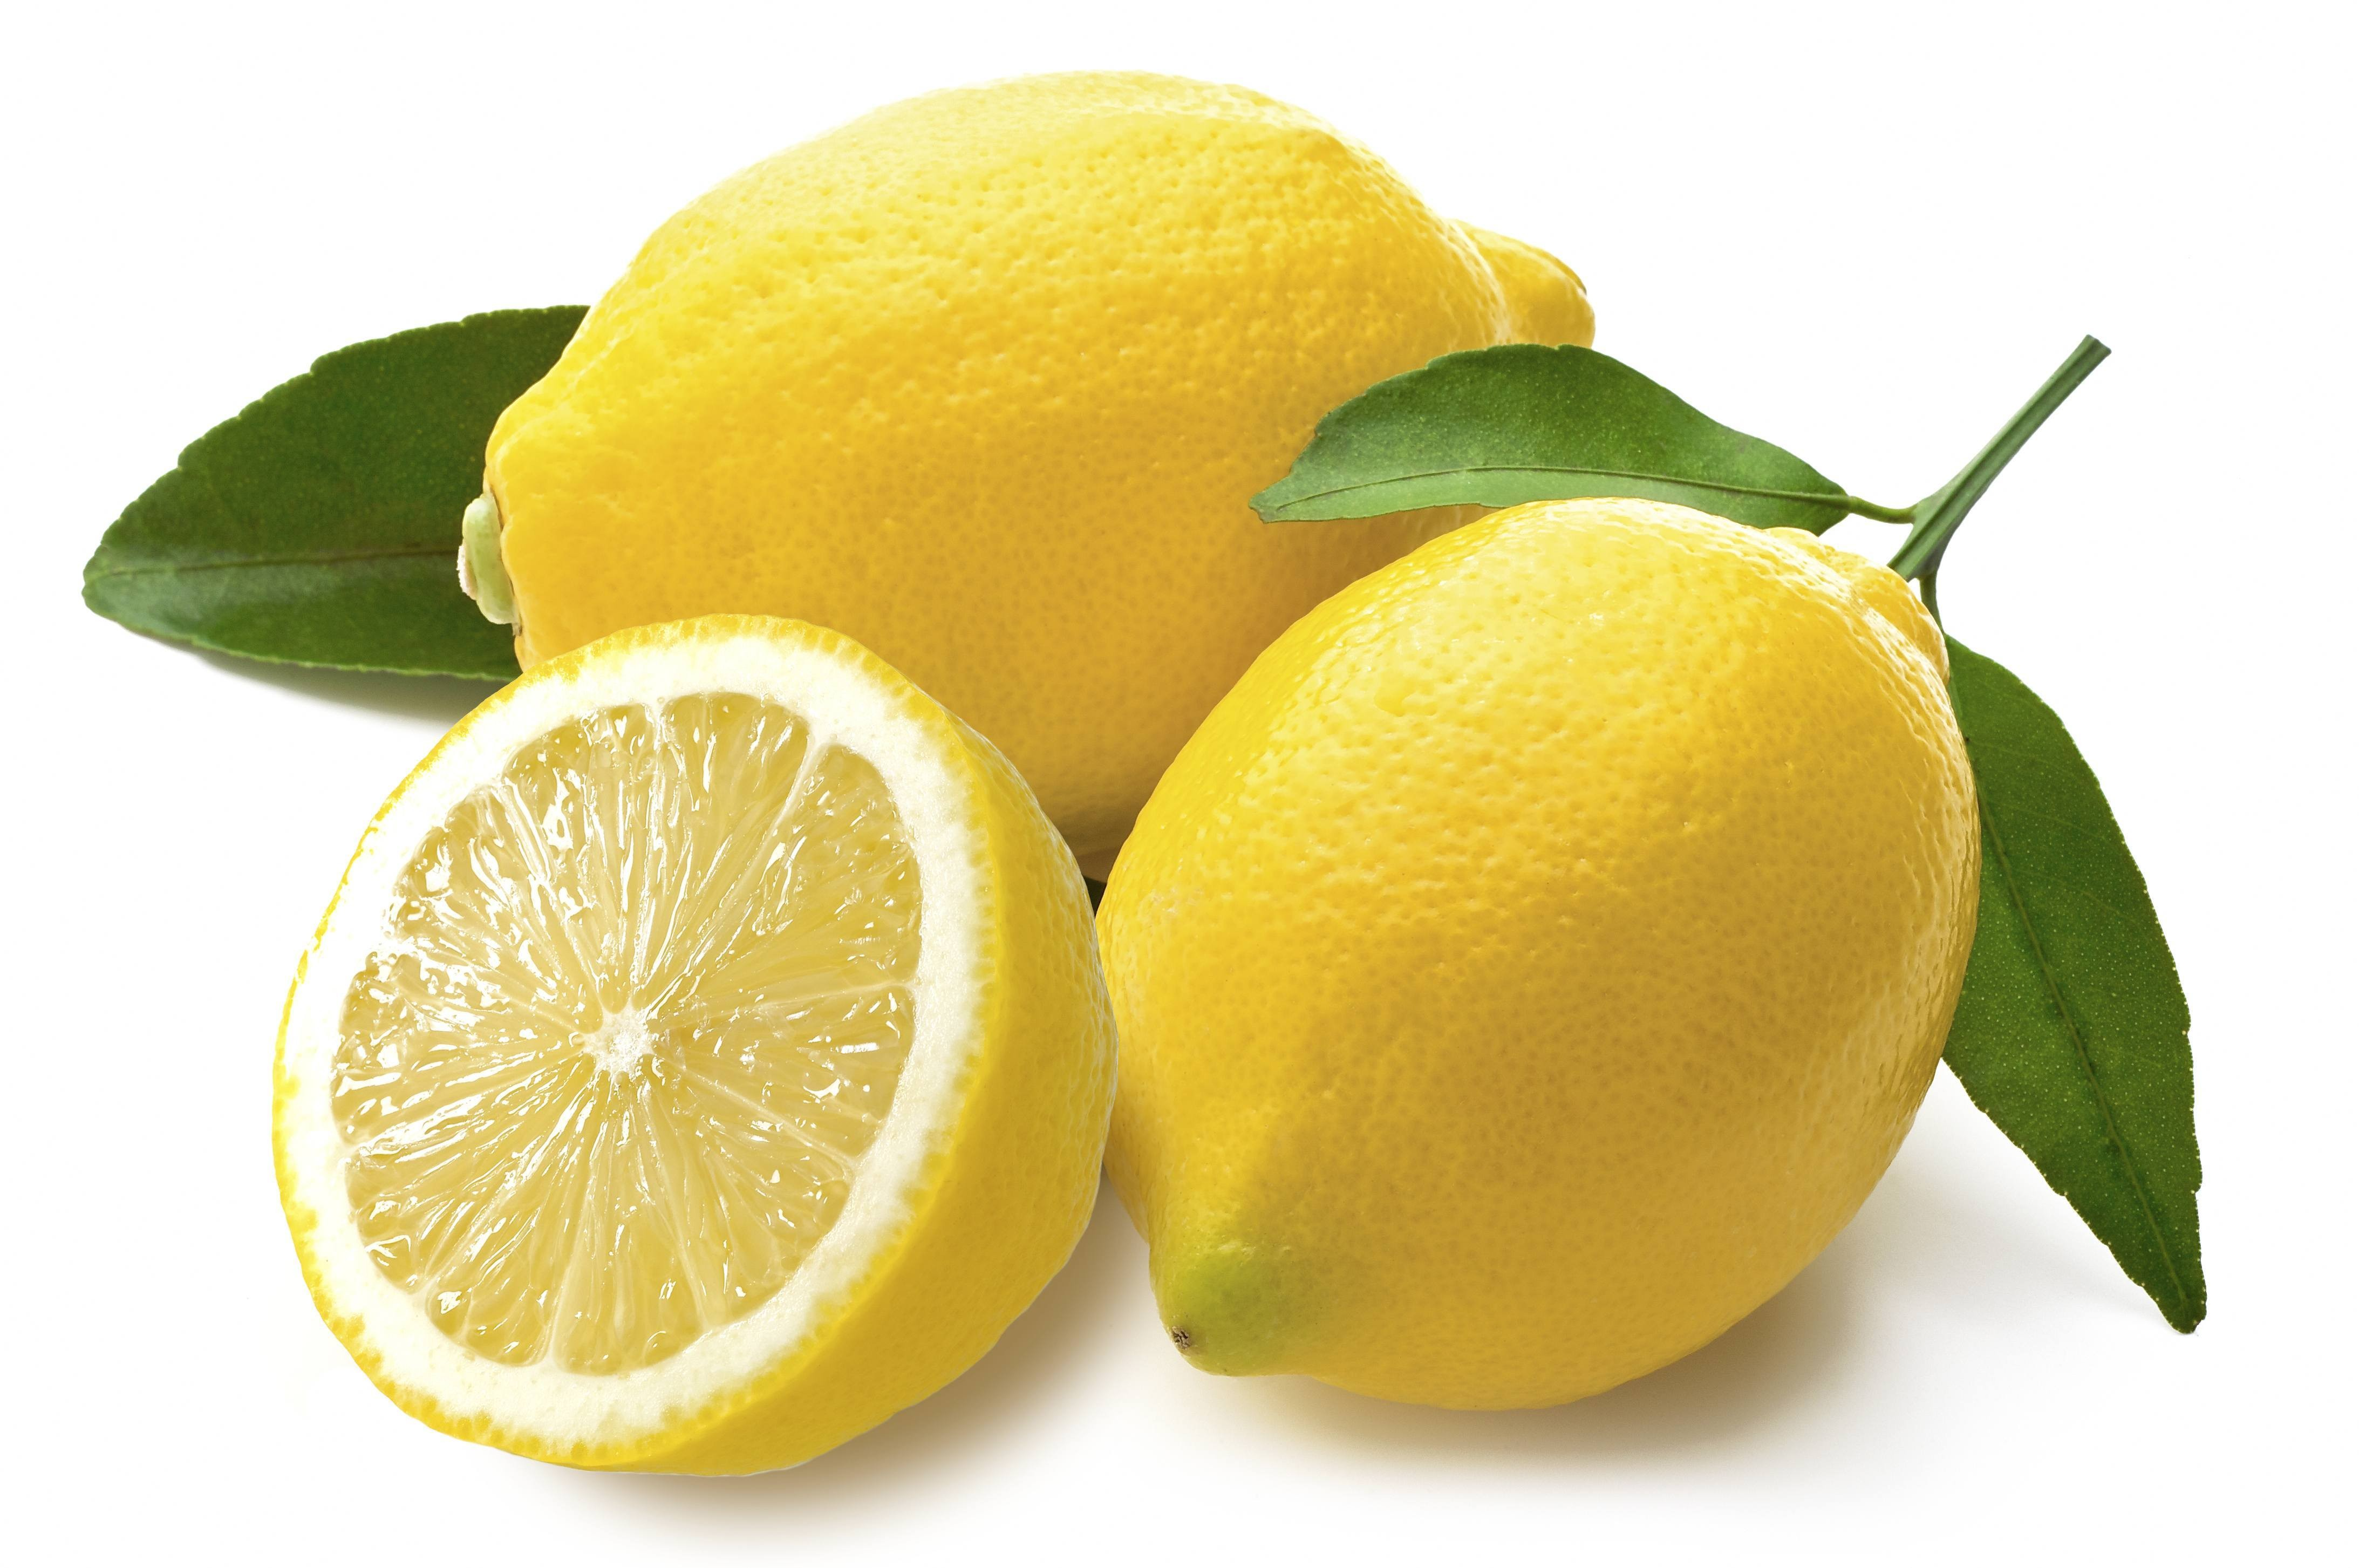
\includegraphics[width=\textwidth]{../img/limon.png}
			\end{figure}

		\end{column}
	\end{columns}
\end{frame}

\begin{frame}[allowdisplaybreaks]
  \frametitle{Svante Arrhenius}
  \begin{columns}
	\begin{column}{.5\textwidth}
	  \begin{itemize}
\item Científico sueco, pionero en la fisicoquímica y galardonado con el Nobel de Química en  1903.
\item Propuso la teoría ácido-base que usamos hasta el día de hoy.
\item Explicó la conductividad eléctrica como resultado de la disociación iónica.
\item Sentó las bases para posteriormente cuantificar la acidez o basicidad de una solución con el pH.
  	  \end{itemize}
	\end{column}

	\begin{column}{.5\textwidth}
\begin{figure}[ht]
  \centering
  \includegraphics[height=.8\textheight]{../img/arrhenius.png}
  \caption{1859 - 1927}
\end{figure}

	\end{column}
  \end{columns}
\end{frame}

\begin{frame}[allowdisplaybreaks]
	\frametitle{Ejemplo. Disociación en agua}
	\begin{columns}
		\begin{column}{.5\textwidth}
			\begin{exampleblock}{Disocie los siguientes ácidos y bases fuertes (disociación completa)}
				\begin{enumerate}
					\item HBr
					\item HI
					\item CsOH
					\item \ce{HNO3}
					\item \ce{H2SO4}
					\item \ce{Ca(OH)2}
				\end{enumerate}
			\end{exampleblock}
		\end{column}
		\begin{column}{.5\textwidth}
		\end{column}
	\end{columns}
\end{frame}

\begin{frame}[allowdisplaybreaks]
	\frametitle{Equilibrio iónico del agua}
	\begin{columns}
		\begin{column}{.5\textwidth}
			\begin{itemize}[<+->]
				\item Si disociamos el \ce{H2O} tenemos: \ce{H2O <=> H+ + OH-}
				\item Entonces: Siempre en una disolución acuosa tendremos iones de \ce{H+} y \ce{OH-}
				\item La cte de equilibrio para el agua (pura) es $K = [\ce{H+}][\ce{OH-}] = \num{1e-14}$
				\item Y en el agua, $[\ce{H+}]=[\ce{OH-}]=\num{1e7}$
			\end{itemize}
		\end{column}

		\begin{column}{.5\textwidth}
			\begin{figure}[ht]
				\centering
				\includegraphics[width=\textwidth]{../img/waterbalance.png}
			\end{figure}

		\end{column}
	\end{columns}
\end{frame}

\begin{frame}[allowdisplaybreaks]
	\frametitle{¿Cómo medir la acidez o basicidad de una solución?}
	\begin{columns}
		\begin{column}{.5\textwidth}
			\begin{itemize}
				\scriptsize
				\item Determinar que tan \textit{ácida} o \textit{básica} es una solución es importante ya que muchos procesos industriales dependen de la cantidad de [\ce{H+}] y [\ce{OH-}].
				\item ¿El problema? Cuando se informan las concentraciones de [\ce{H+}] o [\ce{OH-}] normalmente son valores que rondan 0,000000100 M.
				\item Cifras pequeñas y difíciles de leer. Para superar este problema el científico danés Sørensen (1868-1939) resolvió este problema.
				\item En 1909 mientras trabajaba en la cervecería Carlsen necesitaba comunicar de forma sencilla la acidez y basicidad de la mezcla de cereales.
				\item Y su respuesta fue el pH.
			\end{itemize}
		\end{column}

		\begin{column}{.5\textwidth}
			\begin{figure}[ht]
				\centering
				\includegraphics[height=0.8\textheight]{../img/sorensen.png}
				\caption{Sørensen en su trabajo}
			\end{figure}

		\end{column}
	\end{columns}

\end{frame}

\begin{frame}[allowdisplaybreaks]
	\frametitle{Introducción al concepto de pH: ¿Cómo medir la acidez?}
	\begin{columns}
		\begin{column}{.5\textwidth}
			\begin{itemize}[<+->]
				\item El pH indica la acidez o basicidad de una disolución acuosa.
				\item Se define como: $pH = -\log[\ce{H+}]$
				\item Valores típicos
				      \begin{itemize}[<+->]
					      \item pH < 7 $\rightarrow$ solución ácida.
					      \item pH = 7 $\rightarrow$ neutra.
					      \item pH > 7 $\rightarrow$ básica.
				      \end{itemize}
			\end{itemize}
		\end{column}

		\begin{column}{.5\textwidth}
			\begin{figure}[ht]
				\centering
				\includegraphics[width=\textwidth]{../img/escala-ph.png}
			\end{figure}

		\end{column}
	\end{columns}
\end{frame}

\begin{frame}[allowdisplaybreaks]
	\frametitle{Introducción al concepto de pOH y su relación con el pH}
	\begin{columns}
		\begin{column}{.5\textwidth}
			\begin{itemize}[<+->]
				\item Así como medimos la acidez con el pH, también podemos medir la basicidad con el pOH.
				\item La definición de pOH = $-\log[\ce{OH-}]$
				\item La relación de pH y pOH es inversa, cuando uno aumenta el otro disminuye, ¿Cómo?
			\end{itemize}
		\end{column}

		\begin{column}{.5\textwidth}

		\end{column}
	\end{columns}
\end{frame}

\begin{frame}[allowdisplaybreaks]
	\frametitle{Ejemplo}
	\begin{exampleblock}{Determine el pH y pOH}
		Para una solución:
		\begin{enumerate}
			\item 0,01M de HCl
			\item 0,001M de KOH
			\item 0,005M de \ce{H2SO4} (disociación completa)
			\item 0,005M de \ce{Ca(OH)2} (disociación completa)
		\end{enumerate}

	\end{exampleblock}
\end{frame}

\begin{frame}[allowdisplaybreaks]
	\frametitle{Neutralización Ácido-base}
	\begin{itemize}
		\item ¿Qué sucede cuando un ácido y una base se juntan? se neutralizan
		\item Ejemplo:
		\item \ce{HCl + NaOH -> H2O + NaCl}
		\item Siempre en una neutralización ácido-base, los productos son: un compuesto iónico (sal) y agua.
	\end{itemize}

\end{frame}

\section{Definición del concepto de equilibrio REDOX}

\begin{frame}[allowdisplaybreaks]
	\frametitle{Reacciones de óxido-reducción}
	\begin{columns}
		\begin{column}{.5\textwidth}
			\begin{itemize}[<+->]
				\small
				\item Las reacciones ácido-base tenían como centro, según Arrhenius, liberación de iones \ce{H+} y \ce{OH-}, existen otro tipo de reacciones que, en lugar de cambiar las características del medio, ácido o básico, las podemos usar para producir electricidad.
				\item Esas reacciones se denominan reacciones de óxido-reducción (REDOX)
				\item Y su principal característica es que se describen como una transferencia de electrones dónde una especie pierde (oxida) y otra gana (reduce)
			\end{itemize}
		\end{column}

		\begin{column}{.5\textwidth}
			\ce{Zn(ac) + Cu^{+2}(ac) -> Zn^{+2}(ac) + Cu(ac)}
		\end{column}
	\end{columns}

\end{frame}


\begin{frame}[allowdisplaybreaks]
  \frametitle{Michael Faraday}
  \begin{columns}
	\begin{column}{.5\textwidth}
	  \begin{itemize}
\item Químico/Físico Británico, autodidacta.
\item Estudió junto a Humphry Davy quién hizo grandes aportes al estudio de la electricidad en reacciones químicas.
\item Con los trabajos que continuó encontró las relaciones entre la cantidad de sustancia y la cantidad de carga eléctrica.
\item También introdujo los conceptos de reducción, oxidación, cátodo, ánodo, ión, anión, catión.
	  \end{itemize}
	\end{column}

	\begin{column}{.5\textwidth}
\begin{figure}[ht]
  \centering
  \includegraphics[height=0.8\textheight]{../img/faraday.jpg}
  \caption{1791 - 1867}
\end{figure}

	\end{column}
  \end{columns}

\end{frame}

\section{Determinación de los estados de oxidación de las especies químicas}

\begin{frame}[allowdisplaybreaks]
	\frametitle{Estado de oxidación}
	\begin{columns}
		\begin{column}{.5\textwidth}
			\begin{itemize}
				\item Las especies, como bien estudiamos al inicio del curso, pueden perder, ganar o compartir electrones.
				\item El concepto de estado de oxidación, viene a ser una simplificación de lo anterior.
				\item Asume que dentro de una especie química todos los átomos que la componente, ganan (-) o pierden (+) electrones.
				\item A ese número se le conoce como \textit{estado de oxidación}.
			\end{itemize}
		\end{column}

		\begin{column}{.5\textwidth}
			\begin{itemize}
				\item \ce{CH4}
				\item \ce{CO2}
				\item \ce{NaCl}
				\item \ce{H2}
			\end{itemize}
		\end{column}
	\end{columns}

\end{frame}

\begin{frame}[allowdisplaybreaks]
	\frametitle{Reglas para calcular estados de oxidación}
	\begin{enumerate}
		\item Cada elemento de un compuesto químico presenta su EO.
		\item La suma de los EO es la carga de la especie.
		\item El elemento más electronegativo gana y el menos pierde.
		\item El EO en un elemento, ejemplo \ce{H2} es 0
		\item La mayoría de las veces el O tiene valor -2.
		\item Los metales alcalinos tiene valor de +1.
		\item El H tiene valor de +1 a menos que esté con un metal.
	\end{enumerate}
\end{frame}

\begin{frame}[allowdisplaybreaks]
	\frametitle{Ejemplo}
	\begin{columns}
		\begin{column}{.5\textwidth}
			\begin{exampleblock}{Determine los EO de:}
				\begin{itemize}
					\item \ce{CH4}
					\item \ce{NaOH}
					\item \ce{CH3OH}
					\item \ce{H2SO4}
					\item \ce{Na2ClO4}
				\end{itemize}
			\end{exampleblock}
		\end{column}

		\begin{column}{.5\textwidth}

		\end{column}
	\end{columns}
\end{frame}

\begin{frame}[allowdisplaybreaks]
	\frametitle{Ejemplo 2}
	\begin{exampleblock}{Determine los EO en las siguientes reacciones:}
		\begin{enumerate}
			\small
			\item \ce{4Al + 3O2 -> 2Al2O3}
			\item \ce{2SO2 + O2 -> SO3}
			\item \ce{2CuSO4 + 4KI -> 2CuI + I2 + 2K2SO4}
			\item \ce{H2S + Cl2 -> S + 2HCl}
			\item \ce{3PbO + 2NH3 -> N2 + 3H2O + 3Pb}
		\end{enumerate}

	\end{exampleblock}
\end{frame}

\section{Identificación de las semi reacciones de oxidación, reducción empleando tablas de potenciales de reducción estándares}

\begin{frame}[allowdisplaybreaks]
	\frametitle{Identificación de las semi-reacciones de oxidación y reducción}
	\begin{columns}
		\begin{column}{.5\textwidth}
			\begin{itemize}
				\small
				\item Considere la primera reacción del ejemplo anterior.
				\item \ce{Fe(s) + Cu^{+2}(ac) -> Fe^{+2}(ac) + Cu(s)}
				\item Si se observa bien, podríamos describir lo que le sucedió al hierro y al cobre fue:
				\item \ce{Fe -> Fe^{+2} + 2e-} y
				\item \ce{Cu^{+2} + 2e- -> Cu}
				\item Las reacciones anteriores se denominan semireacciones de oxidación y reducción respectivamente.
			\end{itemize}
		\end{column}

		\begin{column}{.5\textwidth}
			\begin{block}{Conceptos}
				\begin{itemize}
					\item (Agente) reductor
					\item (Agente) oxidante
					\item especie oxidada
					\item especie reducida
					\item electrones transferidos
				\end{itemize}
			\end{block}
		\end{column}
	\end{columns}
\end{frame}

\begin{frame}[allowframebreaks]
	\frametitle{Ejemplo}
	Determine: reductor, oxidante, reducida, oxidada, e- transferidos en las siguientes reacciones:
	\begin{enumerate}
		\item \ce{4Al + 3O2 -> 2Al2O3}
		\item \ce{2SO2 + O2 -> SO3}
		\item \ce{2CuSO4 + 4KI -> 2CuI + I2 + 2K2SO4}
		\item \ce{H2S + Cl2 -> S + 2HCl}
		\item \ce{3PbO + 2NH3 -> N2 + 3H2O + 3Pb}
		\item \ce{3C(s) + 2Fe2O3(s) -> 4Fe(s) + 3CO2(g)}
		\item \ce{Fe2O3(s) + 2 Al(s) -> Al2O3(s) + 2 Fe(l)}
		\item \ce{Cr(s) + 2 HCl(aq) -> CrCl2(aq) + H2(g)}
		\item \ce{SO2(g) + 2 CO(g) -> S(g) + 2 CO2(s)}
		\item \ce{MnO2(s) + 4 HCl(aq) -> MnCl2(aq) + Cl2(g) + 2 H2O(l)}
	\end{enumerate}
\end{frame}

\section{Definición de los conceptos de celdas, cálculo de potenciales normales de reducción y espontaneidad}

\begin{frame}[allowdisplaybreaks]
	\frametitle{Espontaneidad en una reacción Redox}
	\begin{columns}
		\begin{column}{.5\textwidth}
			\begin{itemize}
				\item Las reacciones REDOX implican, como bien revisamos anteriormente, transferencia de e-
				\item Todo flujo de electrones implica un potencial (V) eléctrico $E^{0}_{celda}$.
				\item Según el potencial de la reacción, llamado potencial de celda tenemos tres valores posibles:
				      \begin{itemize}
					      \item $E^{0}_{celda} > 0$: Espontánea
					      \item $E^{0}_{celda} = 0$: Equilibrio
					      \item $E^{0}_{celda} < 0$: No espontánea
				      \end{itemize}
			\end{itemize}
		\end{column}

		\begin{column}{.5\textwidth}
			\begin{block}{Cálculo de potencial}
				\begin{itemize}
					\item $E^{0}_{celda} = E^{0}_{cátodo} - E^{0}_{ánodo}$
					\item $E^{0}_{cátodo}$: Semireacción de reducción.
					\item $E^{0}_{ánodo}$: Semireacción de oxidación.
				\end{itemize}
			\end{block}
		\end{column}
	\end{columns}
\end{frame}



\begin{frame}[allowframebreaks]
	\frametitle{Ejemplo}
	Determine el potencial: cátodo, ánodo, de celda y si será espontánea o no
	\begin{enumerate}
		\item \ce{4Al + 3O2 -> 2Al2O3}
		\item \ce{2SO2 + O2 -> SO3}
		\item \ce{2CuSO4 + 4KI -> 2CuI + I2 + 2K2SO4}
		\item \ce{H2S + Cl2 -> S + 2HCl}
		\item \ce{3PbO + 2NH3 -> N2 + 3H2O + 3Pb}
		\item \ce{3C(s) + 2Fe2O3(s) -> 4Fe(s) + 3CO2(g)}
		\item \ce{Fe2O3(s) + 2 Al(s) -> Al2O3(s) + 2 Fe(l)}
		\item \ce{Cr(s) + 2 HCl(aq) -> CrCl2(aq) + H2(g)}
		\item \ce{SO2(g) + 2 CO(g) -> S(g) + 2 CO2(s)}
		\item \ce{MnO2(s) + 4 HCl(aq) -> MnCl2(aq) + Cl2(g) + 2 H2O(l)}
	\end{enumerate}
\end{frame}


\end{document}
